\documentclass{article}

\usepackage[english]{babel}
\usepackage{amsmath}
\usepackage{amssymb}
\usepackage{amsthm}
\usepackage[font=small]{caption}
\usepackage{cite}
\usepackage{graphicx}

\newtheorem{definition}{Definition}
\newtheorem{example}{Example}
\newtheorem{lemma}{Lemma}
\newtheorem{proposition}{Proposition}
\newtheorem*{remark}{Remark}

%---------------------------------------------------------------

\title{Analytic combinatorics for bioinformatics: applications to
contig assembly and seeding}
\author{
\textsc{Guillaume Filion} \\ [1ex]
\normalsize CRG, Barcelona
}
\date{\today}

%---------------------------------------------------------------
%---------------------------------------------------------------


\begin{document}

\maketitle

\begin{abstract}
Here is the text of the abstract. I need to type more in order to see if
this goes beyond the two columns of the text.
\end{abstract}


%---------------------------------------------------------------
%---------------------------------------------------------------

\section{Introduction}

How many reads should I sequence? How long should they be? With what
minimum overlap? These questions were first addressed in this context by
Lander and Waterman in a landmark study that defined the ``classic
theory'' of assembly \cite{pmid3294162}, giving estimates of the number of
contigs. At the time, genome assembly was a long term endeavour and it
made sense to gather information about the progress of the project. The
Lander-Waterman estimators are thus accurate for intermediate stages where
the number of contigs is high, but their quality drops when the assembly
nears completion.

Nowadays, genome assembly is several orders of magnitude faster. The
questions remain the same, but in many cases the assembly does not have a
proper intermediate stage because the sequencing capacity of a single run
is potentially sufficient to assemble the target genome. It is thus
desirable to minimize the amount of resources that a necessary for the
task, and estimators that are accurate when assembly is likely to be
possible are generally more useful. Likewise, the parameters of the
algorithm must minimize the risk of misassembly while giving the highest
chance that assembly will be possible. This can be done efficiently only
if the statistical properties of the assembly are also understood when it
is likely to be possible.

These are asymptotic estimates, which means that unlike the classical
estimators, they get more accurate when the number of reads increases. In
practice, they are accurate to within 1\% even for a few hundred reads
taken from a genome of a few hunder nucleotides.

All the results shown here are based on original proofs using analytic
combinatorics \cite{AnalComb2009}. The general strategy of analytic
combinatorics is to (i) describe simple combinatorial objects by a
generating function (ii) use simple mathematical operations to find the
generating function of complex structures based on these objects and (iii)
analyze the singularities of the resulting function to derive asymptotic
estimates. This method is sometimes considered counter-intuitive because
generating functions do not directly appeal to intuition
\cite{AnalComb1996}, but it allows to derive precise estimates with simple
proofs.

Since I expect most readers to not be familiar with analytic
combinatorics, I have tried to introduce the ideas progressively, hoping
that the logic of each step will be apparent. This also means that the
information is somewhat spread throughout the manuscript and does not
clearly separate the biological and the mathematical concepts. I have also
tried to use standard notations from analytic combinatorics for the proofs
of the claims, and standard notations from genomic for the specific
applications, which may be slightly confusing.  The key findings are
applications of recent results of Pemantle and Wilson on multivariate
asymptotics. The reader is referred to the original literature for the
proofs of those theorems \cite{PemWil08,AnalComb2013}.

\textbf{Related work:} Schbath and collaborators \cite{pmid10890387}
studied the effect of varying read length on the distribution of contigs.
Wendl \cite{pmid16901236} developed a theory taking into account ``edge
effects'' appearing when the read length is not negligible compared to the
size of the target genome. Stanhope \cite{pmid20686599} studied the
distribution of the largest contig using models of occupancy.


\section{Results}

\subsection{Analytic combinatorics of the assembly problem}
\label{sec:config}

\begin{definition}
If $(a_{k,n})_{k \geq 0, n \geq 0}$ is a bivariate array, the generating
function of the array is by definition

\begin{equation*}
A(x,y) = \sum_{k=0}^\infty \sum_{n=0}^\infty a_{k,n}x^ky^n.
\end{equation*}

When $a_{k,n}$ counts the number of objects in a set $\mathcal{A}$, we
will say that $A(x,y)$ is the generating function of those objects, or the
generating function of $\mathcal{A}$. We will refer to $a_{k,n}$ as the
``coefficient of $x^ky^n$ in $A(x,y)$'', and denote it as ``$[x^ky^n]
A(x,y)$'' whenever convenient.

For convenience, we will call the variable associated to $x$ the
\emph{size} and the variable associated to $y$ the \emph{weight}. The
coefficient of $x^ky^n$ in $A(x,y)$ is thus the number of objects in
$\mathcal{A}$ of size $k$ and weight $n$.
\end{definition}

The function $A$ and the bivariate sequence $(a_{k,n})_{k \geq 0, n \geq
0}$ carry the same information, but some combinatorial operations are
easier to perform with $A$, as we will see below.

The first combinatorial object that we will consider is the ``interval'',
defined here as the distance between the left ends of two consecutive
reads. We will call this distance the size of the interval, and we will
impose it to be a strictly positive integer. This means that two reads
cannot map to the same location, but we will later see how to relax this
constraint. We will also give each interval a weight equal to $1$. This
will later allow us to count intervals when we create more complex
objects.

\begin{figure}[h]
\centering
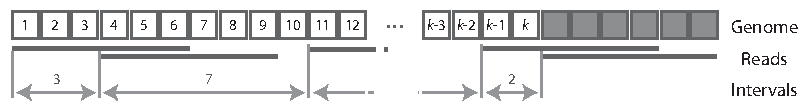
\includegraphics[scale=0.89]{Fig1.pdf}
\caption{\textbf{Representation of the assembly problem}. Here we consider
a single linear chromosome. Reads of identical length are drawn uniformly
without replacement from the chromosome. The distance between the left
ends of consecutive reads forms an interval of requivalent size. We assume
that the leftmost and the rightmost reads always map to the ends of the
chromosome so that intervals always cover exactly $k$ nucleotides.}
\label{fig:sketchass}
\end{figure}

Figure \ref{fig:sketchass} shows the relationships between reads and
intervals. The ``distance'' between two reads will always be the number of
nucleotides between their left ends, which corresponds to an interval of
the same size. Also note that we assume that the leftmost and the
rightmost nucleotides of the genome are exactly covered by reads. This is
not realistic, but such border effects will have negiligible influence on
the asymptotic estimates.

\begin{remark}
In combinatorics, the coverage of $k$ nucleotides by $n$ intervals
corresponds to a \emph{composition}, \textit{i.e.} the break-down of $k$
as a sum of $n$ positive integers \cite{AnalComb2009}.
\end{remark}

The first question of interest is to know the number of different
configurations for a given value of $k$ and $n$. This problem is simple
enough to showcase the methodology of analytic combinatorics, and the
solution will turn out to be very useful. For now, we observe that we can
``construct'' configurations from intervals.

\begin{definition}
A configuration is a sequence of intervals. The generating function of
configurations is denoted $C(x,y)$.
\end{definition}

The general strategy to count configurations will be to find an expression
for $C(x,y)$, extract its coefficients and find asymptotic estimates for
them. For this, we first need to obtain $I(x,y)$, the generating function
of intervals. For $k > 0$ there is exactly one interval of size $k$ and
weight 1, so the coefficient of $x^ky^n$ equals $1$ if $n = 1$ and $k >
0$, and $0$ otherwise. The generating function of intervals is thus

\begin{equation}
\label{eq:F}
I(x,y) = xy + x^2y + x^3y + \ldots
= xy(1+x+x^2+\ldots) = \frac{xy}{1-x}.
\end{equation}

\begin{remark}
Wherever the equality $1+x+x^2+\ldots = 1/(1-x)$ is used, the condition
$|x| < 1$ is assumed to hold.
\end{remark}

Operations on generating functions allow us to create more complex
combinatorial objects. We have already used additions, which correspond
to disjoint unions. For instance, the generating function above says that
an interval is either an interval of size 1 and weight 1, or an interval
of size 2 and weight 1, or an interval of size 3 and weight 1
\textit{etc}. More generally, if $A(x,y)$ and $B(x,y)$ are the generating
functions of objects in disjoint sets $\mathcal{A}$ and $\mathcal{B}$,
then $A(x,y)+B(x,y)$ is the generating function of objects in $\mathcal{A}
\cup \mathcal{B}$.

Multiplications correspond to Cartesian products. More specifically, if
$A(x,y)$ and $B(x,y)$ are the generating functions of objects in sets
$\mathcal{A}$ and $\mathcal{B}$ (disjoint or not), then $A(x,y)B(x,y)$ is
the generating function of objects in $\mathcal{A} \times \mathcal{B}$.
By doing so, we implicitly assume that the size of $(a,b) \in \mathcal{A}
\times \mathcal{B}$ is the size of $a$ plus the size of $b$, and that the
same goes for the weight.

To prove this identity, observe that the pairs of size $k$ and weight $n$
are made of all pairwise combinations of objects whose sizes sum to $k$
and weights sum to $n$. The number of such pairs is $\sum_{l=0}^k
\sum_{m=0}^n a_{l,m}b_{k-l,n-m}$ so the generating function of pairs is

\begin{equation*}
\begin{split}
\sum_{k=0}^\infty &\sum_{n=0}^\infty \left( \sum_{l=0}^k \sum_{m=0}^n
  a_{l,m}b_{k-l,n-m}\right) x^k y^n \\
&= \sum_{l=0}^\infty \sum_{m=0}^\infty \sum_{k=l}^\infty \sum_{n=m}^\infty
  a_{l,m}b_{k-l,n-m}x^{l + k-l} y^{m + n-m} \\ 
&= \sum_{l=0}^\infty \sum_{m=0}^\infty a_{l,m} x^l y^m
  \sum_{k=l}^\infty \sum_{n=m}^\infty
  b_{k-l,n-m}x^{k-l} y^{n-m} \\
&= B(x,y) \sum_{l=0}^\infty \sum_{m=0}^\infty a_{l,m} x^l y^m
 = A(x,y)B(x,y).
\end{split}
\end{equation*}

% Explain that the size just counts the intervals.
By taking both $\mathcal{A}$ and $\mathcal{B}$ as the set of intervals, we
see that the generating function of pairs of intervals is $I(x,y)^2$.
Applying this formula multiple times, we also see that $I(x,y)^n$ is the
generating function of sequences of $n$ of intervals. Since a sequence of
intervals is either a sequence of $0$ interval, or a sequence of $1$
interval, or a sequence of $2$ intervals \textit{etc}., we can write the
generating function of configurations as

\begin{equation*}
C(x,y) = \sum_{n=0}^\infty \left( \frac{xy}{1-x} \right)^n
= \frac{1}{1 - xy/(1-x)}.
\end{equation*}

\begin{remark}
Note that a sequence of $n$ intervals has weight $n$, so the weight is a
proxy for the number of intervals in the configuration.  We say that $y$
``marks'' the number of intervals.
\end{remark}

We have used $I(x,y)$ to obtain an algebraic expression for $C(x,y)$. The
coefficient of $x^ky^n$ in $C(x,y)$ is the number of configurations where
$n$ intervals cover $k$ nucleotides, but its value does not appear
spontaneously. Fortunately, we can write $C(x,y)$ in such a way that it
will become more obvious. Observe that

\begin{equation}
\label{eq:C}
C(x,y) = \frac{1-x}{1-x(1+y)} =
(1-x) \sum_{k=0}^\infty \left(x(1+y) \right)^k.
\end{equation}


Using Newton's binomial formula, we can expand $(1+y)^k$ so as to extract
the powers of $y$, namely

\begin{equation*}
C(x,y) = (1-x)\sum_{k=0}^\infty x^k\sum_{n=0}^k {k \choose n} y^n
= \sum_{k=0}^\infty\sum_{n=0}^\infty{k \choose n} (x^ky^n - x^{k+1}y^n).
\end{equation*}

It follows that

\begin{equation}
\label{eq:coefC}
[x^ky^n] C(x,y) =
{k \choose n} - {k-1 \choose n} = {k-1 \choose n-1}
\text{, provided $k > 0$, $n > 0$}.
\end{equation}

It can also be seen that the cases $k = 0$ and $n = 0$ give coefficients
equal to $0$, except for $k = n = 0$ where the coefficient is equal to
$1$.

\begin{remark}
The last expression in (\ref{eq:C}) gives an alternative construction for
sequences of intervals. The term $1+y$ is the generating function of bits,
\textit{i.e.} elements of $\{0,1\}$, so $(x(1+y))^k$ is the generating
function of bit strings where $x$ marks the size and $y$ marks the number
of bits set to $1$. To exhibit a bijection we can encode left ends of
intervals with a $1$ and every other position with a $0$. The factor $1-x$
is a correction for the fact that the first bit is always set to $1$ (see
Figure \ref{fig:sketchass}).
\end{remark}

We now have the \emph{exact} number of configurations for every value of
$k$ and $n$. To obtain asymptotic estimates, we can use Stirling's formula
$n! \sim n^ne^{-n}\sqrt{2\pi n}$. After cancellations we see that the
number of configurations is asymptotically equivalent to

\begin{equation}
\label{eq:assBC}
[x^ky^n]C(x,y) \sim \frac{k^{k-1}}{n^{n-1}(k-n)^{k-n}}
\sqrt{\frac{k}{2\pi n(k-n)}}.
\end{equation}

A more direct approach would have been to observe that a configuration is
a draw of $n-1$ left ends among $k-1$ positions, leading directly to
(\ref{eq:coefC}). The benefit of the analytic combinatorics approach is
that we can now tinker the generating function $C(x,y)$ to obtain results
that do not lend themselves to such direct approaches.




%%%%%%%%%%%%% Average number of contigs %%%%%%%%%%%%%
\subsection{Average number of contigs}
\label{sec:av}

Some configurations are better than others for the purpose of assembling
the genome. In order to investigate the properties of ``good''
configurations, we need to introduce new combinatorial objects.

\begin{definition}
A $d$-interval is an interval of size no greater than $d$ and a $d$-gap is
an interval of size greater than $d$. The generating function of
$d$-intervals is denoted $I_d(x,y)$ and the generating function of
$d$-gaps is denoted $G_d(x,y)$.
\end{definition}

Intuitively, if two reads are separated by a $d$-interval, it will be
possible to merge them, whereas if they are separated by a $d$-gap this
will not be possible. The value of $d$ depends on the concrete assembly
problem at hand and on the read length ($d$ is higher for longer reads).
This natually lead to the following definition.

\begin{definition}
\label{def:contig}
A contig is a non-empty sequence of $d$-intervals. The generating function
of contigs is denoted $K(x,y)$.
\end{definition}

\begin{figure}[h]
\centering
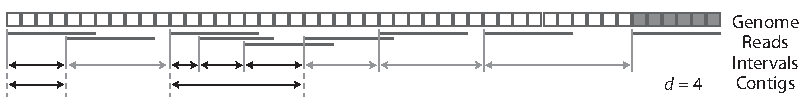
\includegraphics[scale=0.9]{Fig2.pdf}
\caption{\textbf{Contigs and gaps}. In this example $d=4$, so contigs
correspond to sequences of one of more $4$-intervals. The color of the
double arrow is black for $4$-intervals and grey for $4$-gaps. The
configuration contains two contigs.}
\label{fig:contigs}
\end{figure}

In real assembly problems, there is no guarantee that merging consecutive
reads will be possible every time their distance is no greater than some
threshold $d$. Because of sequencing errors, repeated sequences and other
practical complications, the number of contigs on real problems is
systematically lower than on ideal problems.

It is interesting to estimate the number of contigs that one may expect to
obtain. Instead of jumping directly to this task, we will count $d$-gaps
instead. This will be useful for exposition purposes, and the answer will
bring some insight into the assembly problem.

Following the strategy of analytic combinatorics, we must first find the
generating functions of the objects under focus. Going back to the
construction of intervals, we can see that the generating functions of
$d$-intervals and $d$-gaps are

\begin{equation*}
\begin{split}
I_d(x,y) &= yx + yx^2 + \ldots + yx^d = yx\frac{1-x^d}{1-x}\text{, and} \\
G_d(x,y) &= yx^{d+1} + yx^{d+2} + \ldots = y\frac{x^{d+1}}{1-x}.
\end{split}
\end{equation*}

Observe that $I_d(x,y)+G_d(x,y) = I(x,y)$ because an interval is either a
$d$-interval or a $d$-gap (and because the intersection of $d$-intervals
and $d$-gaps is empty). Using this, we can write the generation of
configurations as

\begin{equation}
\label{eq:C2ndform}
C(x,y) = \sum_{n=0}^\infty I(x,y)^n
= \sum_{n=0}^\infty \left( I_d(x,y) + G_d(x,y) \right)^n.
\end{equation}

Since $d$-gaps appear explicitly in this expression of $C(x,y)$, we can
use another variable, say $u$, to mark them. For this, we just have to
multiply their generating function $G_d(x,y)$ by $u$ so that every time a
$d$-gap appears in a configuration, the exponent of $u$ is raised by $1$.
The same method was applied earlier to let $y$ mark the number of
intervals. Transforming $C(x,y)$ as proposed, we obtain


\begin{equation*}
H(x,y,u) = \sum_{n=0}^\infty \left(xy\frac{1-x^d}{1-x} +
uy\frac{x^{d+1}}{1-x}\right)^n
= \frac{1-x}{1-x-y\left(x(1-x^d) +ux^{d+1}\right)}.
\end{equation*}

$H(x,y,u)$ is the generating function of a three-dimensional array
$(a_{k,n,m})$, where each term is the number of configurations of total
size $k$, total weight $n$ and with $m$ $d$-gaps. Note that both
$d$-intervals and $d$-gaps contribute to the weight, so that it still
indicates the number of intervals. For a given value of $k$ and $n$, the
cumulative number of $d$-gaps is $\sum_{m=0}^\infty ma_{k,n,m}$. Since for
the same values of $k$ and $n$ the total number of configurations is
$\sum_{m=0}^\infty a_{k,n,m}$ the average number of $d$-gaps is

\begin{equation}
\label{eq:average}
\sum_{m=0}^\infty ma_{k,n,m}\Big/\sum_{m=0}^\infty a_{k,n,m}.
\end{equation}

As usual, we will find the generating functions of the numerator and the
denomiator of (\ref{eq:average}) and extract their respective
coefficients. Observe that

\begin{equation*}
\begin{split}
\frac{\partial H(x,y,u)}{\partial u}\Bigr|_{\substack{\\u=1}} &=
\sum_{k=0}^\infty\sum_{n=0}^\infty
\left(\sum_{m=0}^\infty ma_{k,n,m}\right) x^ky^n \text{, and} \\
H(x,y,1) &= \sum_{k=0}^\infty\sum_{n=0}^\infty
\left(\sum_{m=0}^\infty a_{k,n,m} \right)x^ky^n.
\end{split}
\end{equation*}

It is easier to start with the generating function of the denominator as
the results are already available. Equation (\ref{eq:C2ndform}) says that
$H(x,y,1) = C(x,y)$. This is intuitive, because counting $d$-gaps should
not change the total number of configurations. Now turning to the
numerator we obtain

\begin{equation*}
\frac{\partial H(x,y,u)}{\partial u}\Bigr|_{\substack{\\u=1}}
= \frac{yx^{d+1}(1-x)}{\left(1-x(1+y)\right)^2}.
\end{equation*}

There is no obvious way to extract the coefficients of this generating
function. Fortunately, it is close to another generating function for
which we already know the coefficients. Observe that

\begin{equation*}
\frac{\partial C(x,y)}{\partial y} = 
\frac{x(1-x)}{\left(1-x(1+y)\right)^2}.
\end{equation*}

So $\partial H(x,y,u)/\partial u|_{\substack{\\u=1}} = yx^d\partial
C(x,y)/\partial y$ and the coefficient of $x^ky^n$ in the generating
function of the numrator of (\ref{eq:average}) is $n[x^{k-d}y^n]C(x,y)$.
The average number of $d$-gaps is thus

\begin{equation*}
n {k-d-1 \choose n-1} \Big/ {k-1 \choose n-1}.
\end{equation*}

For $k < d$ or $n > k-d$ the average number of gaps is $0$.  We can also
use equation (\ref{eq:assBC}) or Sitrling's formula to obtain a simple
asymptotic estimate for the expected number of $d$-gaps, namely

\begin{equation*}
n\left(1-n/k\right)^d.
\end{equation*}

\begin{remark}
Here the benefits of the analytic combinatorics approach become obvious.
It is much more difficult to tink of a direct approach leading to the same
results.
\end{remark}

Recall that this formula assumes that reads cannot map to the same
location. It is possible to filter out identical reads, but it would be
useful to relax this constraint in order to compute estimates before any
data is acquired.

For this, let us assume that there is a total of $n_*$ reads drawn
\emph{with} replacement. Each nucleotide of the chromosome corresponds to
the left end of a read $n_*/k$ times on average. Because $k$ and $n_*$ are
both large, we can approximate the number of time a nucleotide is drawn by
a Poisson distribution with mean $n_*/k$. The probability that a position
is the left end of a read is approximately $1-e^{-n_*/k}$, so $n \approx
k(1-e^{-n_*/k})$.

\begin{remark}
Allowing intervals and $d$-intervals to have size $0$ is not the proper
way to address this issue because it gives different sampling
probabilities.  For $4$ reads covering $2$ nucleotides the probability
that the first two intervals have size $0$ would be $1/3$, whereas it
should be $2/7$.
\end{remark}

The asymptotic estimate for the expected number of gaps as a function of
the chromosome size $k$ and the number of reads $n_*$ is

\begin{equation}
\label{eq:avstar}
k(1-e^{-n_*/k})e^{-dn_*/k}.
\end{equation}

Expression (\ref{eq:avstar}) is useful because at high coverage there will
be approximately one $d$-gap between every pair of contigs, so we can
estimate of the average number of contigs as $1 + k(1-e^{-n_*/k})
e^{-dn_*/k}$. However, at low coverage this estimate is inaccurate
because there will be many consecutive $d$-gaps not enclosing a contig.

For the general case, we need to count contigs in a slightly more tedious
way. The function $H(x,y,u)$ above is a ``counting function'' and $u$ is
the ``counting parameter''. We can count contigs by decorating their
generating function with $u$ and again compute their average number
through the ratio

\begin{equation*}
\frac{[x^ky^n] \partial H(x,y,u)/\partial u|_{\substack{\\u=1}}}
{[x^ky^n]H(x,y,1)}.
\end{equation*}

All we need to do is to find a way to ``construct'' configurations from
contigs and apply the same method as above. It is intuitively clear that
configurations are composed of contigs and of non-empty sequences of
$d$-gaps, so we need to find the generating functions of those objects.
Contigs are non-empty sequences of $d$-intervals, so their generating
function is

\begin{equation*}
K(x,y) = \sum_{n=1}^\infty \left( F_d(x,y) \right)^n
= \sum_{n=1}^\infty \left(yx\frac{1-x^d}{1-x} \right)^n
= \frac{yx(1-x^d)/(1-x)}{1-yx(1-x^d)/(1-x)}.
\end{equation*}

Similarly, denoting $G(x,y)$ the generating function of non-empty
sequences of $d$-gaps, we can express it as

\begin{equation*}
G(x,y) = \sum_{n=1}^\infty \left(G_d(x,y) \right)^n
= \sum_{n=1}^\infty \left(y\frac{x^{d+1}}{1-x} \right)^n
= \frac{yx^{d+1}/(1-x)}{1-yx^{d+1}/(1-x)}.
\end{equation*}

Now, the basic unit of configurations is a non-empty contig followed by a
non-empty sequence of $d$-gaps, whose generating function is
$uK(x,y)G(x,y)$. The presence of $u$ here indicates that each unit adds 1
to the count of contigs. A configuration is a sequence of such units, but
it starts with a potentially empty sequence of $d$-gaps, whose generating
function is $1+G(x,y)$, and it ends with a potentially empty contig, whose
generating function is $1+uK(x,y)$. The counting function thus comes out
as

\begin{equation*}
\begin{split}
H(x,y,u) &= \left( 1+G(x,y) \right)
\left( \sum_{n=0}^\infty (uK(x,y)G(x,y))^n \right)
\left( 1+uK(x,y) \right) \\
& = \frac{(1+G(x,y))(1+uK(x,y))}{1-uK(x,y)G(x,y)}.
\end{split}
\end{equation*}

One can check from the definitions of $K(x,y)$ and $G(x,y)$ that $H(x,y,1)
= C(x,y)$ as expected. Again, the derivative of $H(x,y,1)$ is related to
$C(x,y)$, and following the same strategy as above, we obtain

\begin{equation*}
\partial H(x,y,u)/\partial u|_{\substack{\\u=1}}
= y(1-x^d)\left( 1 - y(x+\ldots+x^d) \right)
\frac{\partial C(x,y)}{\partial y}.
\end{equation*}

The relationship between the coefficients of $\partial H(x,y,u) /\partial
u|_{\substack{\\u=1}}$ and those of $C(x,y)$ is more cumbersome than for
$d$-gaps, but we still obtain an exact expression for the exepected number
of contigs, namely

\begin{equation*}
\begin{split}
\Bigg[ n{k-1 \choose n-1} - &n{k-d-1 \choose n-1} -
(n-1){k-2 \choose n-2} - \ldots - (n-1) {k-d-1 \choose n-2} +
\\ &(n-1){k-d-2 \choose n-2} +
\ldots + (n-1){k-2d-1 \choose n-2} \Bigg] \Big/ {k-1 \choose n-1}.
\end{split}
\end{equation*}

More interesting is the asymptotic estimate, which comes in a
simpler form. The formula above is asymptotically equal to

\begin{equation}
\label{eq:avcont}
\left( 1+n(1-n/k)^d \right) \left(1-(1-n/k)^d\right).
\end{equation}

We recognize ur previous estimator
$1+n(1-n/k)^d$, but here it is corrected by the factor $1-(1-n/k)^d$,
which speicifically declines at low coverage.

Using the Poisson approximation, we can again express the expected number
of contigs as a function of the total number of reads as

\begin{equation}
\label{eq:avcontnstar}
(1 + k(1-e^{-n_*/k})e^{-dn_*/k} ) (1-e^{-dn_*/k}).
\end{equation}

Let us now examine a concrete example. In Figure~\ref{fig:avcontig} we
consider a small genome of $k = 25,000$ nucleotides, where contigs are
composed of $24$-intervals. We measure the average number of contigs over
$100,000$ random samples for different number of reads $n$ and compare
this value to the Lander-Waterman estimate $ne^{-dn/k}$, to the Roach
estimate $1+(n-1)(1-d/k)^n$, and to the estimate given by formula
(\ref{eq:avcontnstar}).


\begin{figure}[h]
\centering
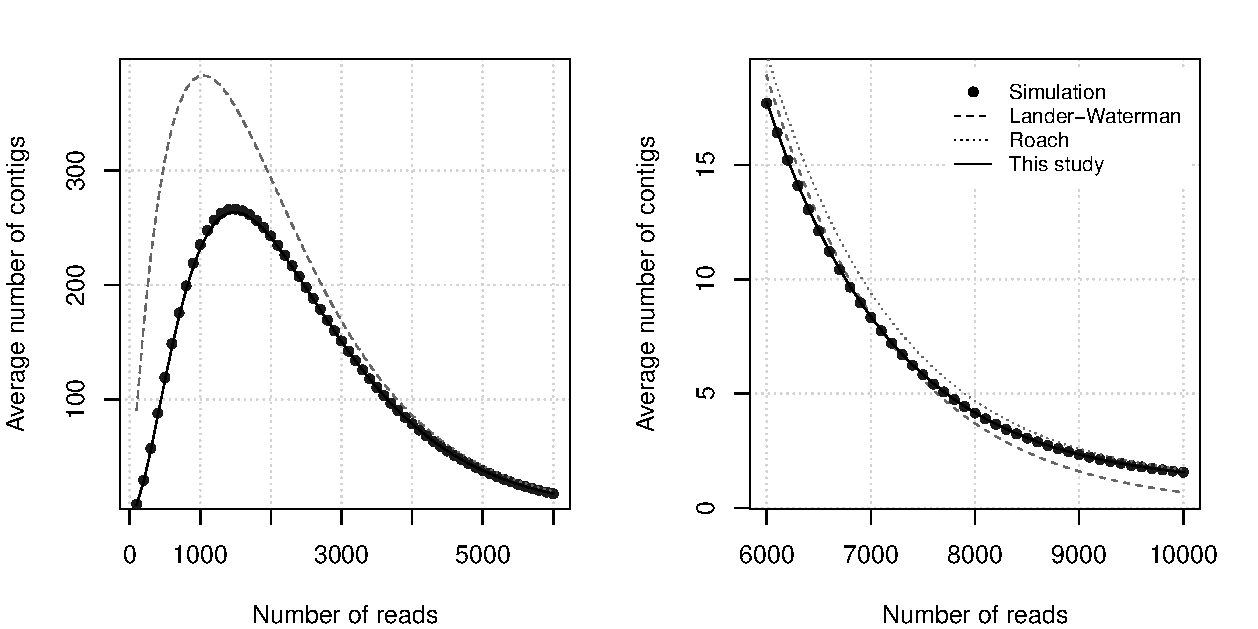
\includegraphics[scale=0.585]{Fig3.pdf}
\caption{\textbf{Average number of contigs}. In this example, $k=25,000$
and $d=24$. Between $100$ and $10,000$ reads were drawn at random with
replacement and the number of contigs was calculated following definition
\ref{def:contig}. Each case was replicated $100,000$ times and the average
was plotted (circles). Dotted lines show the Lander-Waterman and Roach
estimates (the lines are superimposed in the left panel) and the plain
lines show the estimate computed from expression (\ref{eq:avcontnstar}).
The lander-Waterman and Roach estimates are sustantially biased at low
read count (left panel). At high read count (right panel), the Roach
estimate is asymptotically unbiased, but the Lander-Waterman estimate is
not. Here the estimate of this study never deviates by more than 2\%.}
\label{fig:avcontig}
\end{figure}

It is clear that formula (\ref{eq:avcontnstar}) is the most accurate,
especially at low number of reads. The absolute error is largest at the
maximum number of contigs (around $1500$ reads), where the estimate is too
small by approximately $3$ contigs. The relative error is largest at the
lowest number of reads, where it is 5\% too low. Above $2000$ reads the
relative error is below 1\% (in comparison, the relative error of the
Roach estimate never drops below 8\% on this data). These small
differences do not disppear for larger values of $k$, they are due to the
Poisson approximation used to turn expression (\ref{eq:avcont}) into
(\ref{eq:avcontnstar}), which brings small but systematic biases.

In conclusion, we have obtained an estimator that is accurate at all
values of the coverage. It is important to highlight that it derives from
the standard analytic combinatorics and that it involves only basic
mathematical manipulations.




%%%%%%%%%%%%% Average contig size %%%%%%%%%%%%%
\subsection{Average contig size}

It is interesting to compute the average size of the contigs. All the
tools that we need to obtain an estimate have already been introduced.

The simplest strategy is to compute the cumulative size of $d$-gaps and
get the cumulative size of contigs by complementarity. We can exhibit a
counting function for the size of $d$-gaps and derive asymptotic estimates
using the same strategy as in the previous section. All we have to do is
mark the size of a $d$-gaps with corresponding powers of $u$. In
expression (\ref{eq:C2ndform}), $G_d(x,y)$ will be replaced by 
$y(x^{d+1}u^{d+1} + x^{d+2}u^{d+2} + \ldots ) = yx^{d+1}u^{d+1}/(1-xu)$.
The counting function for the size of $d$-gaps is thus

\begin{equation*}
\begin{split}
H(x,y,u) &= \sum_{n=0}^\infty \left(yx\frac{1-x^d}{1-x} +
y\frac{x^{d+1}u^{d+1}}{1-xu}\right)^n \\
&= \frac{1}{1-y \left(x(1-x^d)/(1-x) +
x^{d+1}u^{d+1}/(1-xu) \right)}.
\end{split}
\end{equation*}

Once again, it is easy to check that $H(x,y,1) = C(x,y)$. Differentiating
with respect to $u$, we obtain

\begin{equation*}
\frac{\partial H(x,y,u)}{\partial u}\Bigr|_{\substack{\\u=1}}
= y \frac{(d+1)x^{d+1}-dx^{d+2}}{(1-x)^2} \frac{\partial C(x,y)}
{\partial y}.
\end{equation*}

This yields an exact expression for the cumulative size of $d$-gaps
averaged over all configurations\footnote{This result is somewhat more
technical than the previous ones and it requires the equality
$(k+1){k \choose n} + k{k-1 \choose n} + \ldots = (n+1){k+2
\choose n+2}$.}

\begin{equation}
(d+1)n {k-d \choose n+1} -dn {k-d-1 \choose n+1}.
\end{equation}


This is asymptotically equivalent to $k(1-n/k)^{d+1}(d+k/n)$.  Since the
expected asymptotic number of $d$-gaps is $n(1-n/k)^d$, we see that their
individual size is asymptotic to $(k/n-1)(d+k/n)$. Intuitively, the size
of $d$-gaps is very large when $n$ is much smaller than $k$.

We can also compute the expected unassembled fraction, \textit{i.e.} the
fraction of nucleotides covered by $d$-gaps. For this we just have to
divide the cumulative size of $d$-gaps by the total size $k$ and we obtain
$(1-n/k)^{d+1}(d+k/n)$.

To answer the original question, we compute the total size of contigs by
complementary as $k-k(1-n/k)^{d+1}(d+k/n)$. Now dividing by the
average number of contigs, we find that the expected asymptotic size as

\begin{equation}
\frac{k(1-(1-n/k)^{d+1}(d+k/n))}
{\left(1+n(1-n/k)^d\right)\left(1-(1-n/k)^d \right)}.
\end{equation}

This expression is somewhat cumbersome, but it becomes approximately equal
to $k/(1+n(1-n/k)^d)$ when $n$ is close to $k$. This quantity expressed in
terms of raw number of reads is

\begin{equation}
\frac{k\left( 1-e^{-(d+1)n_*/k}(d+1/(1-e^{-n_*/k})) \right)}
{( 1 + k(1-e^{-n_*/k})e^{-dn_*/k}) (1-e^{-dn_*/k})}.
\end{equation}

Similarly, when $n_*$ is of the order of $k$, this expression becomes
approximately equal to $k/(1+ke^{-dn_*/k}(1-e^{-n_*/k}))$.







%%%%%%%%%%%%%%%%%%%%%%%%%%%%
\subsection{Probability of closure}
\label{sec:compass}

Riordan arrays are bivariate arrays $(a_{k,n})_{k,n}$ such that the
generating function satisfies

\begin{equation*}
\sum_{k=0}^\infty \sum_{n=0}^\infty a_{k,n} x^k y^n =
\frac{\phi(x)}{1-y \nu(x)}.
\end{equation*}

\begin{proposition}
\label{th:PW}
Assume that $F(x,y)$ is the generating function of a Riordan array, and
that $k$ and $n$ tend to infinity with $\lim k/n = \lambda$, then

\begin{equation}
\label{eq:assRA}
[x^ky^n]F(x,y) \sim \frac{\nu(x_\lambda)^n\phi(x_\lambda)}
  {x_\lambda^k\sqrt{2\pi n \sigma(x_\lambda)^2}},
\end{equation}

\noindent
where $x_\lambda$ is the solution of $\mu(x) = x\nu'(x)/\nu(x) = \lambda$
and where $\sigma(x)^2 = x \mu'(x)$.
\end{proposition}

In essence, proposition \ref{th:PW} says that if $k \sim \lambda n$ and if
we can find the solution of the equation $\mu(x) = \lambda$, then we get
the asymptotic growth of the Riordan array $a_{k,n}$. The proof of this
theorem is outside the scope of this article; interested readers are
referred to the original results of Pemantle and Wilson
\cite{PemWil02,AnalComb2013}.

Expression (\ref{eq:C}) shows that $C(x,y)$ is the generating function of
a Riordan array with $\phi(x) = 1$ and $\nu(x) = x/(1-x)$.  Here $\mu(x) =
1/(1-x)$ and $\sigma^2(x) = x/(1-x)^2$, so we obtain $x_\lambda = (\lambda
-1)/\lambda$, $\nu(x_\lambda) = \lambda -1$, and $\sigma^2(x_\lambda) =
\lambda(\lambda-1)$. Combining this with $\lambda \sim k/n$ we obtain

% This is where I define tight coverage.
In the shotgun strategy of genome assembly, reads are merged if they
overlap by some minimum amount of nucleotides. The process continues with
consecutive reads in both directions, as long as they overlap by this
minimum amount of nucleotides. The merged sequences are called
\emph{contigs}, and the assembly of a chromosome is theoretically possible
if it consists of a single contig (in practice, the fact that biological
sequences are interspersed with repeats makes assembly more difficult). We
call this event ``tight coverage'', and it is interesting to determine
its \textit{a priori} probability.

From here on, $d$ will denote the maximal allowed distance between the
left ends of consecutive reads that can be merged. Note that the minimum
amount of nucleotides that reads must overlp is $L-d$, where $L$ is their
length. We also introduce intervals of size no greater than $d$ and call
them ``$d$-intervals''. Since the case $d=1$ is trivial, we will assume $d
> 1$ throughout.

Following the same rationale as bove, we first need to find the generating
function of $d$-intervals. This is done easily by stopping the sum in
(\ref{eq:F}) after $x^dy$, so we obtain $F_d(x,y) = (x+x^2+\ldots+x^d)y$.
Since a contig is a sequence of $d$-intervals, the generating function of
contigs is

\begin{equation}
\label{eq:Cd}
C_d(x,y) = \sum_{n=0}^\infty \left(y(x+x^2+\ldots+x^d)\right)^n =
\frac{1}{1-y(x+x^2+\ldots+x^d)}.
\end{equation}

The coefficients of $C_d(x,y)$ are known as the polynomial coefficients,
but they cannot be expressed in closed form. However, this is not an issue
because (\ref{eq:Cd}) is the generating function of a Riordan with
$\phi(x) = 1$ and $\nu(x) = x + x^2 + \ldots + x^d$, so we can extract
their asymptotic behavior from proposition \ref{th:PW}.

\begin{lemma}
\label{th:mu}
For $\nu(x) = x+x^2+\ldots+x^d$, the equation $\mu(x) = x\nu'(x)/\nu(x) =
\lambda$ has a single solution $x_\lambda$ for $1 \leq \lambda \leq d$.
\end{lemma}

\begin{proof}
We first demonstrate that for $x \geq 0$, $\mu$ is strictly increasing.
This will ensure that if the solution is unique if it exists.

\begin{equation}
\label{eq:mu}
\mu(x) = x\frac{\nu'(x)}{\nu(x)} =
\frac{x+2x^2+3x^3+\ldots+dx^d}{x+x^2+\ldots+x^d} =
d+\frac{1}{1-x} - \frac{d}{1-x^d}.
\end{equation} 

Differentiating the last expression we obtain

\begin{equation}
\label{eq:muprime}
\mu'(x) = \frac{1}{(1-x)^2} -\frac{d^2x^{d-1}}{(1-x^d)^2}.
\end{equation}

The function $f(\alpha) = x^{\alpha} = e^{\alpha \log(x)}$ is strictly
convex for every $x > 0$ and $x \neq 1$. Applying the definition of
convexity, we obtain the inequality

\begin{eqnarray*}
\frac{f(0)+\ldots+f(d-1)}{d} &>&
f\left(\frac{0+1+2+\ldots+d-1}{d}\right) \\
\frac{1+x+\ldots+x^{d-1}}{d} &>& f\left(\frac{d-1}{2}\right)
= x^{(d-1)/2} \\
\frac{1-x^d}{1-x} &>& dx^{(d-1)/2} \\
\frac{1}{(1-x)^2} &>& \frac{d^2x^{d-1}}{(1-x^d)^2}.
\end{eqnarray*}

Combined with equation (\ref{eq:muprime}), the last inequality shows that
$\mu'(x) > 0$ for $x > 0$ and $x \neq 1$. Since $\mu'(0) = 1$ and $\mu'(1)
= (d+1)(d-1)/12$, $\mu$ is strictly increasing (note that $\mu'(1)$ is
properly defined but that $\mu'(0)$ must be defined by continuity).
Observing that $\mu(0) = 1$ and $\lim_{x\rightarrow\infty} \mu(x) = d$,
the equation $\mu(x) = \lambda$ has a unique solution provided $1 \leq
\lambda \leq d$.
\end{proof}

\begin{remark}
The cases $\lambda > d$ and $\lambda < 1$ correspond to limits where $k >
nd$ and $k < n$, respectively. Since the size of a collection of $n$
$d$-intervals is between $n$ and $nd$, we have the trivial asymptotic
behavior $a_{k,n} = 0$ in both cases.
\end{remark}


The value of $x_\lambda$ can be found numerically using expression
(\ref{eq:mu}).  Once it is available, we can compute $\nu(x_\lambda)$ and
$\sigma(x_\lambda^2)$ from their definitions, but numeric precision can
become an issue if $n$ or $d$ is very large. To avoid this, we can use the
equivalent expressions


\begin{gather}
\label{eq:nu} %% Equation for nu.
\nu(x_\lambda) = \frac{dx_\lambda}{1+(d-\lambda)(1-x_\lambda)}, \\
\label{eq:sigma} %% Equation for sigma2.
\sigma(x_\lambda)^2 = \lambda(d-\lambda) -
  \frac{d-2\lambda+1}{1-x_\lambda}.
\end{gather}

The coefficients of $C(x,y)$ give the total number of configurations, and
those of $C_d(x,y)$ give the number of configurations with a single
contig. The probability that a chromosome can be assembled is thus
$[x^ky^n] C_d(x,y) / [x^ky^n] C(x,y)$, which can be approximated with the
asymptotic formulas developed above.

\begin{example}
Let us consider a genome of size 25,001. We assume that 10,001 reads are
drawn uniformly at random without replacement. This translates into
$k=25000$ and $n=10000$. Setting the maximum distance between reads in a
contig to $d=25$, what is the probability that the genome can be
assembled?

First, we get $\lambda = k/n = 2.5$. We then solve equation (\ref{eq:mu})
with the Newton-Raphson method and obtain $x_\lambda \approx 0.600011377$.
Using equations (\ref{eq:nu}) and (\ref{eq:sigma}) we obtain
$\nu(x_\lambda) \approx 1.50006684$ and $\sigma(x_\lambda)^2 \approx
3.747554$. We compute equation (\ref{eq:assRA}) in logarithmic space and
obtain

\begin{equation*}
\begin{split}
10000&\log(1.50006684) - 25000\log(0.600011377) \\
- &\log(10000)/2 - \log(3.747554)/2 - \log(2\pi)/2
\approx 16819.0786.
\end{split}
\end{equation*}

We also compute 

\begin{equation*}
\log { 24999 \choose 9999 } \approx 16819.1067.
\end{equation*}

The estimated probability that a configuration corresponds to a coverage
by $25$-intervals is thus

\begin{equation*}
\exp(16819.0783-16819.1067) \approx 0.972.
\end{equation*}

Randomly sampling 200,000 configurations gives an estimate for this
probability equal to $0.972$, close to the numerical approximation by
three digits. In this example, $x_\lambda$ and $\nu(x_\lambda)$ must be
approximated to eight digits in order to obtain an approximate accurate to
within 1\%. Using the definition of $\nu$ instead of (\ref{eq:nu}), we
would obtain an estimate equal to $0.983$. The difference is negligible
here, but on real problems, $n$ and $k$ can be several orders of magnitude
higher, which will increase the difference.
\end{example}

In the above, we have assumed that all the reads map to different
locations. It is possible to enforce this by removing duplicate reads, but
it would be more useful to estimate the probability that the chromosome
can be assembled before resources are spent. 

Assume that there is a total of $n_*$ reads and that they are drawn with
replacement. Each nucleotide of the chromosome corresponds to the left end
of a read $n_*/k$ times on average. Because $k$ and $n$ are both large, we
can approximate the number of time a nucleotide is drawn by a Poisson
distribution with mean $n_*/k$. The probability that a position is not
sampled is approximately $e^{-n_*/k}$ so that the frequency of sampled
positions is $1-e^{-n_*/k}$. The strategy is thus to replace the true
number of reads by the expected number of distinct reads

\begin{equation}
\label{eq:nstar}
n = k(1-e^{-n_*/k}).
\end{equation}


\begin{example}
We consider the same problem as in the previous example, with a genome of
size 25,001 and 10,001 reads at a maximum distance of 25 ncleotides, but
this time the reads are drawn uniformly at random with replacement. As
above, $k=25000$, but we need to replace $n$ by $25000 \cdot
(1-e^{-10000/25000}) \approx 8241.9988$.

We now obtain $\lambda = k/n \approx 3.033$. Following the same
calculations as in the previous example, we obtain $x_\lambda \approx
0.67044394$, $\nu(x_\lambda) \approx 2.03429230$ and
$\sigma(x_\lambda)^2 \approx 6.144599$. Computing (\ref{eq:assRA}) in
logarithmic space with the new values yields

\begin{equation*}
\begin{split}
8241.9988\log(2.03429230) - &25000\log(0.67044394) \\
- \log(8241.9988)/2 - &\log(6.144599)/2 - \log(2\pi)/2
\approx 15842.084.
\end{split}
\end{equation*}

Likewise, we also have

\begin{equation*}
\log { 24999 \choose 8240.9988 } \approx 15842.457.
\end{equation*}

Finally, the estimated probability that a configuration corresponds to a
coverage by $25$-intervals is

\begin{equation*}
\exp(15842.084-15842.457) \approx 0.689.
\end{equation*}

Randomly sampling 200,000 configurations gives an estimate for this
probability equal to $0.688$. This is less accurate than in the previous
example, but still within 1\% of the real value.
\end{example}

In conclusion, we can continue to assume that reads are all distinct, and
use formula (\ref{eq:nstar}) whenever the assumption does not hold.

\begin{remark}
Allowing intervals and $d$-intervals to have size $0$ is not the proper
way to address this issue because it gives a different sampling scheme.
For $4$ reads covering $2$ nucleotides (\textit{i.e.} $k=1$ and $n=3$),
the probability that the first two intervals have size $0$ would be $1/3$,
whereas it should be $2/7$.
\end{remark}

In summary, estimates of the chances of success of the assembly are
accurate in the range where they are the most useful, namely when the
value is not exceedingly close to 0 or to 1. The steps required to
automate the estimation are recapitulated here:

\begin{enumerate}
\item Compute the expected number of distinct reads $n$ using
(\ref{eq:nstar}). 
\item Compute $\lambda = k/n$.
\item Solve $\mu(x_\lambda) = \lambda$ by the Newton-Raphson method using
(\ref{eq:mu}) and (\ref{eq:muprime}).
\item Compute $\nu(x_\lambda)$ and $\sigma^2(x_\lambda)$ using
(\ref{eq:nu}) and (\ref{eq:sigma}).
\item Compute (\ref{eq:assRA}) in logarithmic space.
\item Compute (\ref{eq:coefC}) in logarithmic space.
\item Take the difference of the last two terms and exponentiate.
\end{enumerate}



\section{Discussion}

Strictly speaking, we do not need the theorems by Pemantle and Wilson.
Here we care only about approximations rather than asymptotics. We could
have used earlier results by Drmota \cite{Drmota1994} or Gardy
\cite{Gardy1995}, or we could have used the saddle point asymptotics
method on $(x(1-x^d)/(1-x))^n$ we would obtain expression (\ref{eq:assRA})
for fixed $n$ and $k$, which is sufficient for our purpose. However, this
would have required to check that the function satisfies some conditions
that are fairly technical. Proposition \ref{th:PW} is very general and it
makes this step unnecessary.

%---------------------------------------------------------------
%---------------------------------------------------------------

\bibliography{pubmed,extra}
\bibliographystyle{plain}

%----------------------------------------------------------------

\end{document}
